\documentclass[10pt,ignorenonframetext,]{beamer}
\setbeamertemplate{caption}[numbered]
\setbeamertemplate{caption label separator}{: }
\setbeamercolor{caption name}{fg=normal text.fg}
\beamertemplatenavigationsymbolsempty
\usepackage{lmodern}
\usepackage{amssymb,amsmath}
\usepackage{ifxetex,ifluatex}
\usepackage{fixltx2e} % provides \textsubscript
\ifnum 0\ifxetex 1\fi\ifluatex 1\fi=0 % if pdftex
\usepackage[T1]{fontenc}
\usepackage[utf8]{inputenc}
\else % if luatex or xelatex
\ifxetex
\usepackage{mathspec}
\else
\usepackage{fontspec}
\fi
\defaultfontfeatures{Ligatures=TeX,Scale=MatchLowercase}
\fi
% use upquote if available, for straight quotes in verbatim environments
\IfFileExists{upquote.sty}{\usepackage{upquote}}{}
% use microtype if available
\IfFileExists{microtype.sty}{%
\usepackage{microtype}
\UseMicrotypeSet[protrusion]{basicmath} % disable protrusion for tt fonts
}{}
\newif\ifbibliography
\usepackage{color}
\usepackage{fancyvrb}
\newcommand{\VerbBar}{|}
\newcommand{\VERB}{\Verb[commandchars=\\\{\}]}
\DefineVerbatimEnvironment{Highlighting}{Verbatim}{commandchars=\\\{\}}
% Add ',fontsize=\small' for more characters per line
\usepackage{framed}
\definecolor{shadecolor}{RGB}{248,248,248}
\newenvironment{Shaded}{\begin{snugshade}}{\end{snugshade}}
\newcommand{\KeywordTok}[1]{\textcolor[rgb]{0.13,0.29,0.53}{\textbf{{#1}}}}
\newcommand{\DataTypeTok}[1]{\textcolor[rgb]{0.13,0.29,0.53}{{#1}}}
\newcommand{\DecValTok}[1]{\textcolor[rgb]{0.00,0.00,0.81}{{#1}}}
\newcommand{\BaseNTok}[1]{\textcolor[rgb]{0.00,0.00,0.81}{{#1}}}
\newcommand{\FloatTok}[1]{\textcolor[rgb]{0.00,0.00,0.81}{{#1}}}
\newcommand{\ConstantTok}[1]{\textcolor[rgb]{0.00,0.00,0.00}{{#1}}}
\newcommand{\CharTok}[1]{\textcolor[rgb]{0.31,0.60,0.02}{{#1}}}
\newcommand{\SpecialCharTok}[1]{\textcolor[rgb]{0.00,0.00,0.00}{{#1}}}
\newcommand{\StringTok}[1]{\textcolor[rgb]{0.31,0.60,0.02}{{#1}}}
\newcommand{\VerbatimStringTok}[1]{\textcolor[rgb]{0.31,0.60,0.02}{{#1}}}
\newcommand{\SpecialStringTok}[1]{\textcolor[rgb]{0.31,0.60,0.02}{{#1}}}
\newcommand{\ImportTok}[1]{{#1}}
\newcommand{\CommentTok}[1]{\textcolor[rgb]{0.56,0.35,0.01}{\textit{{#1}}}}
\newcommand{\DocumentationTok}[1]{\textcolor[rgb]{0.56,0.35,0.01}{\textbf{\textit{{#1}}}}}
\newcommand{\AnnotationTok}[1]{\textcolor[rgb]{0.56,0.35,0.01}{\textbf{\textit{{#1}}}}}
\newcommand{\CommentVarTok}[1]{\textcolor[rgb]{0.56,0.35,0.01}{\textbf{\textit{{#1}}}}}
\newcommand{\OtherTok}[1]{\textcolor[rgb]{0.56,0.35,0.01}{{#1}}}
\newcommand{\FunctionTok}[1]{\textcolor[rgb]{0.00,0.00,0.00}{{#1}}}
\newcommand{\VariableTok}[1]{\textcolor[rgb]{0.00,0.00,0.00}{{#1}}}
\newcommand{\ControlFlowTok}[1]{\textcolor[rgb]{0.13,0.29,0.53}{\textbf{{#1}}}}
\newcommand{\OperatorTok}[1]{\textcolor[rgb]{0.81,0.36,0.00}{\textbf{{#1}}}}
\newcommand{\BuiltInTok}[1]{{#1}}
\newcommand{\ExtensionTok}[1]{{#1}}
\newcommand{\PreprocessorTok}[1]{\textcolor[rgb]{0.56,0.35,0.01}{\textit{{#1}}}}
\newcommand{\AttributeTok}[1]{\textcolor[rgb]{0.77,0.63,0.00}{{#1}}}
\newcommand{\RegionMarkerTok}[1]{{#1}}
\newcommand{\InformationTok}[1]{\textcolor[rgb]{0.56,0.35,0.01}{\textbf{\textit{{#1}}}}}
\newcommand{\WarningTok}[1]{\textcolor[rgb]{0.56,0.35,0.01}{\textbf{\textit{{#1}}}}}
\newcommand{\AlertTok}[1]{\textcolor[rgb]{0.94,0.16,0.16}{{#1}}}
\newcommand{\ErrorTok}[1]{\textcolor[rgb]{0.64,0.00,0.00}{\textbf{{#1}}}}
\newcommand{\NormalTok}[1]{{#1}}
\usepackage{graphicx,grffile}
\makeatletter
\def\maxwidth{\ifdim\Gin@nat@width>\linewidth\linewidth\else\Gin@nat@width\fi}
\def\maxheight{\ifdim\Gin@nat@height>\textheight0.8\textheight\else\Gin@nat@height\fi}
\makeatother
% Scale images if necessary, so that they will not overflow the page
% margins by default, and it is still possible to overwrite the defaults
% using explicit options in \includegraphics[width, height, ...]{}
\setkeys{Gin}{width=\maxwidth,height=\maxheight,keepaspectratio}

% Prevent slide breaks in the middle of a paragraph:
\widowpenalties 1 10000
\raggedbottom

\AtBeginPart{
\let\insertpartnumber\relax
\let\partname\relax
\frame{\partpage}
}
\AtBeginSection{
\ifbibliography
\else
\let\insertsectionnumber\relax
\let\sectionname\relax
\frame{\sectionpage}
\fi
}
\AtBeginSubsection{
\let\insertsubsectionnumber\relax
\let\subsectionname\relax
\frame{\subsectionpage}
}

\setlength{\parindent}{0pt}
\setlength{\parskip}{6pt plus 2pt minus 1pt}
\setlength{\emergencystretch}{3em}  % prevent overfull lines
\providecommand{\tightlist}{%
\setlength{\itemsep}{0pt}\setlength{\parskip}{0pt}}
\setcounter{secnumdepth}{0}

\title{R Tutorial}
\author{Brad Setzler}
\institute{University of Chicago}
\date{July, 2018}

\begin{document}
\frame{\titlepage}

\begin{frame}
\tableofcontents[hideallsubsections]
\end{frame}

\begin{frame}

\end{frame}

\begin{frame}[fragile]{Preliminaries}

To complete this tutorial, you will need to download and install:

\begin{itemize}
\tightlist
\item
  R (\url{https://www.r-project.org/})
\item
  RStudio (\url{https://www.rstudio.com/})
\end{itemize}

Once R is installed, run these commands to install useful packages:

\small

\begin{Shaded}
\begin{Highlighting}[]
\KeywordTok{install.packages}\NormalTok{(}\StringTok{"data.table"}\NormalTok{) }\CommentTok{# big data management}
\KeywordTok{install.packages}\NormalTok{(}\StringTok{"ggplot2"}\NormalTok{) }\CommentTok{# graphing}
\KeywordTok{install.packages}\NormalTok{(}\StringTok{"lfe"}\NormalTok{) }\CommentTok{# fixed effects models}
\KeywordTok{install.packages}\NormalTok{(}\StringTok{"AER"}\NormalTok{) }\CommentTok{# IV regressions}
\KeywordTok{install.packages}\NormalTok{(}\StringTok{"styler"}\NormalTok{) }\CommentTok{# code style}
\KeywordTok{install.packages}\NormalTok{(}\StringTok{"devtools"}\NormalTok{) }\CommentTok{# package development}
\KeywordTok{install.packages}\NormalTok{(}\StringTok{"roxygen2"}\NormalTok{) }\CommentTok{# package documentation}
\KeywordTok{install.packages}\NormalTok{(}\StringTok{"testthat"}\NormalTok{) }\CommentTok{# testing tools}
\end{Highlighting}
\end{Shaded}

\normalsize

\small

\begin{verbatim}
## Warning: package 'data.table' was built under R version 3.3.2
\end{verbatim}

\begin{verbatim}
## Warning: package 'ggplot2' was built under R version 3.3.2
\end{verbatim}

\normalsize

\end{frame}

\begin{frame}[fragile]{Frequently Asked Questions}

Before getting into R, here are the answers to the questions I have
heard the most about it:

\begin{enumerate}
\def\labelenumi{\arabic{enumi}.}
\tightlist
\item
  Is R a full programming language? \emph{Yes.}
\item
  Is R popular? \emph{Yes, it is the \#10 most popular language, per
  TIOBE.}
\item
  In R code, do \texttt{a=1} and \texttt{a\textless{}-1} mean the same
  thing? \emph{Yes.}
\item
  In R code, do \texttt{a=\textquotesingle{}hello\textquotesingle{}} and
  \texttt{a="hello"} mean the same thing? \emph{Yes.}
\item
  Can R be used for purposes other than statistical applications?
  \emph{Yes, this LaTeX presentation was created by R.}
\end{enumerate}

\end{frame}

\section{I. Introduction to 4 Workhorse
Objects}\label{i.-introduction-to-4-workhorse-objects}

\begin{frame}{Overview: 4 Workhorse Objects}

This section will demonstrate the basics of working with 4 common
objects in R:

\begin{enumerate}
\def\labelenumi{\arabic{enumi}.}
\tightlist
\item
  vector;
\item
  data.table;
\item
  function; and,
\item
  list.
\end{enumerate}

\end{frame}

\begin{frame}[fragile]{Workhorse Objects in R (1/4): vector}

A \emph{vector} is defined with the \texttt{c()} operator. Arithmetic
operations are applied element-wise:

\footnotesize

\begin{Shaded}
\begin{Highlighting}[]
\NormalTok{a_vector <-}\StringTok{ }\KeywordTok{c}\NormalTok{(}\DecValTok{1}\NormalTok{, }\DecValTok{2}\NormalTok{, }\DecValTok{8}\NormalTok{)}
\NormalTok{a_vector *}\StringTok{ }\DecValTok{3} \NormalTok{/}\StringTok{ }\DecValTok{2} \NormalTok{+}\StringTok{ }\DecValTok{4}
\end{Highlighting}
\end{Shaded}

\begin{verbatim}
## [1]  5.5  7.0 16.0
\end{verbatim}

\normalsize

Once a vector has a string, all contents are converted to strings:

\footnotesize

\begin{Shaded}
\begin{Highlighting}[]
\NormalTok{another_vector <-}\StringTok{ }\KeywordTok{c}\NormalTok{(}\DecValTok{1}\NormalTok{, }\FloatTok{2.5}\NormalTok{, }\StringTok{"hello"}\NormalTok{)}
\KeywordTok{print}\NormalTok{(another_vector)}
\end{Highlighting}
\end{Shaded}

\begin{verbatim}
## [1] "1"     "2.5"   "hello"
\end{verbatim}

\normalsize

\end{frame}

\begin{frame}[fragile]{Workhorse Objects in R (2/4): data.table}

A \emph{data.table} is a powerful data structure in R. We will study its
various capabilities in the next section. Here, we only show here how to
construct a \texttt{data.table} and add a column to it:

\footnotesize

\begin{Shaded}
\begin{Highlighting}[]
\KeywordTok{library}\NormalTok{(data.table)}
\NormalTok{a_data_table <-}\StringTok{ }\KeywordTok{data.table}\NormalTok{(}\DataTypeTok{year =} \KeywordTok{c}\NormalTok{(}\DecValTok{1}\NormalTok{, }\DecValTok{1}\NormalTok{, }\DecValTok{2}\NormalTok{, }\DecValTok{2}\NormalTok{), }\DataTypeTok{value =} \KeywordTok{rnorm}\NormalTok{(}\DecValTok{4}\NormalTok{))}
\NormalTok{a_data_table[, person :}\ErrorTok{=}\StringTok{ }\KeywordTok{c}\NormalTok{(}\StringTok{"John"}\NormalTok{, }\StringTok{"Mary"}\NormalTok{, }\StringTok{"John"}\NormalTok{, }\StringTok{"Mary"}\NormalTok{)]}
\NormalTok{a_data_table}
\end{Highlighting}
\end{Shaded}

\begin{verbatim}
##    year       value person
## 1:    1 -2.19887302   John
## 2:    1 -0.93627678   Mary
## 3:    2  0.04338172   John
## 4:    2 -0.70776538   Mary
\end{verbatim}

\normalsize

\end{frame}

\begin{frame}[fragile]{Workhorse Objects in R (3/4): function}

A \emph{function} takes inputs (which must be named, separated by
commas, and may be assigned default values using the equals sign) and
returns an output:

\footnotesize

\begin{Shaded}
\begin{Highlighting}[]
\NormalTok{a_function <-}\StringTok{ }\NormalTok{function(arg1, }\DataTypeTok{arg2 =} \FloatTok{3.5}\NormalTok{) \{}
  \NormalTok{intermediate <-}\StringTok{ }\NormalTok{arg1 +}\StringTok{ }\NormalTok{arg2}
  \NormalTok{final <-}\StringTok{ }\NormalTok{intermediate^}\FloatTok{2.5}
  \KeywordTok{return}\NormalTok{(final)}
\NormalTok{\}}

\KeywordTok{a_function}\NormalTok{(}\DecValTok{2}\NormalTok{) }\CommentTok{# using the default arg2 value}
\end{Highlighting}
\end{Shaded}

\begin{verbatim}
## [1] 70.94254
\end{verbatim}

\begin{Shaded}
\begin{Highlighting}[]
\KeywordTok{a_function}\NormalTok{(}\DecValTok{2}\NormalTok{, }\DecValTok{7}\NormalTok{) }\CommentTok{# overriding the default arg2 value}
\end{Highlighting}
\end{Shaded}

\begin{verbatim}
## [1] 243
\end{verbatim}

\normalsize

\end{frame}

\begin{frame}[fragile]{Workhorse Objects in R (4/4): list}

A \emph{list} is the most general type of R object, which may include
any other type of R object as an element with a string as the key:

\tiny

\begin{Shaded}
\begin{Highlighting}[]
\NormalTok{a_list <-}\StringTok{ }\KeywordTok{list}\NormalTok{(}
  \StringTok{"a vector"} \NormalTok{=}\StringTok{ }\NormalTok{a_vector,}
  \StringTok{"a data.table"} \NormalTok{=}\StringTok{ }\NormalTok{a_data_table,}
  \StringTok{"a function"} \NormalTok{=}\StringTok{ }\NormalTok{a_function}
\NormalTok{)}

\NormalTok{a_list}
\end{Highlighting}
\end{Shaded}

\begin{verbatim}
## $`a vector`
## [1] 1 2 8
## 
## $`a data.table`
##    year       value person
## 1:    1 -2.19887302   John
## 2:    1 -0.93627678   Mary
## 3:    2  0.04338172   John
## 4:    2 -0.70776538   Mary
## 
## $`a function`
## function (arg1, arg2 = 3.5) 
## {
##     intermediate <- arg1 + arg2
##     final <- intermediate^2.5
##     return(final)
## }
\end{verbatim}

\normalsize

\end{frame}

\begin{frame}[fragile]{Workhorse Objects in R: Putting all 4 objects
together}

\tiny

\begin{Shaded}
\begin{Highlighting}[]
\NormalTok{combined_function <-}\StringTok{ }\NormalTok{function(a.list, }\DataTypeTok{flag =} \NormalTok{F) \{}
  \NormalTok{func1 <-}\StringTok{ }\NormalTok{function(arg}\FloatTok{.1}\NormalTok{, arg}\FloatTok{.2}\NormalTok{) \{}
    \NormalTok{dt <-}\StringTok{ }\KeywordTok{data.table}\NormalTok{(}\DataTypeTok{results =} \KeywordTok{c}\NormalTok{(arg}\FloatTok{.1}\NormalTok{, arg}\FloatTok{.2}\NormalTok{) /}\StringTok{ }\DecValTok{2}\NormalTok{)}
    \NormalTok{dt[, arg :}\ErrorTok{=}\StringTok{ }\KeywordTok{c}\NormalTok{(}\DecValTok{1}\NormalTok{, }\DecValTok{2}\NormalTok{)]}
    \KeywordTok{return}\NormalTok{(dt)}
  \NormalTok{\}}

  \NormalTok{func2 <-}\StringTok{ }\NormalTok{function(arg}\FloatTok{.1}\NormalTok{, arg}\FloatTok{.2}\NormalTok{) \{}
    \KeywordTok{return}\NormalTok{(arg}\FloatTok{.1} \NormalTok{-}\StringTok{ }\NormalTok{arg}\FloatTok{.2}\NormalTok{)}
  \NormalTok{\}}

  \NormalTok{arg1 <-}\StringTok{ }\NormalTok{a.list[[}\StringTok{"first argument"}\NormalTok{]]}
  \NormalTok{arg2 <-}\StringTok{ }\NormalTok{a.list[[}\StringTok{"second argument"}\NormalTok{]]}

  \NormalTok{output <-}\StringTok{ }\OtherTok{NULL}
  \NormalTok{if (flag) \{}
    \NormalTok{output <-}\StringTok{ }\KeywordTok{func1}\NormalTok{(arg1, arg2)}
  \NormalTok{\}}
  \NormalTok{if (!flag) \{}
    \NormalTok{output <-}\StringTok{ }\KeywordTok{func2}\NormalTok{(arg1, arg2)}
  \NormalTok{\}}

  \KeywordTok{return}\NormalTok{(output)}
\NormalTok{\}}

\NormalTok{this_list <-}\StringTok{ }\KeywordTok{list}\NormalTok{(}\StringTok{"first argument"} \NormalTok{=}\StringTok{ }\FloatTok{2.0}\NormalTok{, }\StringTok{"second argument"} \NormalTok{=}\StringTok{ }\FloatTok{3.5}\NormalTok{)}

\KeywordTok{print}\NormalTok{(}\KeywordTok{combined_function}\NormalTok{(this_list, }\DataTypeTok{flag =} \NormalTok{T))}
\end{Highlighting}
\end{Shaded}

\begin{verbatim}
##    results arg
## 1:    1.00   1
## 2:    1.75   2
\end{verbatim}

\normalsize

\end{frame}

\begin{frame}[fragile]{Quiz \#1: Workhorse Objects in R}

Write a function with 3 arguments:

\begin{itemize}
\tightlist
\item
  The first argument is the vector \texttt{temperature} (no default);
\item
  The second argument is the boolean \texttt{FtoC} (default
  \texttt{FtoC=TRUE});
\item
  The third argument is the list \texttt{options} (no default).
\end{itemize}

This function does the following:

\begin{itemize}
\tightlist
\item
  Converts temperature from Fahrenheit to Celsius if \texttt{FtoC=T};
\item
  Converts temperature from Celsius to Fahrenheit if \texttt{FtoC=F};
\item
  If there is not an argument in \texttt{options} called
  \texttt{option1}, it prints an error to the screen that says
  \texttt{"error:\ options\$option1\ must\ exist"} {[}hint: use the
  \texttt{stop()} command{]}.
\item
  Returns a \texttt{data.table} with Celsius and Fahrenheit columns.
\end{itemize}

Provide examples that work as expected when \texttt{FtoC=TRUE} and when
\texttt{FtoC=FALSE}, and with/without including \texttt{option1} in
\texttt{options}.

\end{frame}

\section{II. Data Analysis, Visualization, and
Import/Export}\label{ii.-data-analysis-visualization-and-importexport}

\begin{frame}{Overview}

This section shows how to analyze panel data in R:

\begin{enumerate}
\def\labelenumi{\arabic{enumi}.}
\tightlist
\item
  Simulating panel data from a given DGP;
\item
  Computing aggregate statistics;
\item
  Plotting bivariate relationships;
\item
  OLS and fixed effect regressions;
\item
  Constructing lags and differences; and,
\item
  Importing/exporting results.
\end{enumerate}

We will rely on data.table throughout.

\end{frame}

\begin{frame}[fragile]{Simulation in data.table}

Suppose we wish to simulate panel data \((Y_{i,t},X_{i,t})\) from the
DGP:

\[
Y_{i,t} = \alpha + \beta X_{i,t} + t\kappa  + \mu_i + \epsilon_{i,t}, \quad \epsilon_{i,t} \sim_{iid} \mathcal{N}(0,\sigma^2)
\]

where \(X\) depends on \(\mu\) and \(t\) (more on this later). It can be
simulated as:

\footnotesize

\begin{Shaded}
\begin{Highlighting}[]
\KeywordTok{library}\NormalTok{(data.table)}
\KeywordTok{set.seed}\NormalTok{(}\DecValTok{101}\NormalTok{) }\CommentTok{# Always set the seed before simulating data}
\NormalTok{NI <-}\StringTok{ }\DecValTok{1000} \CommentTok{# Number of individuals}
\NormalTok{NT <-}\StringTok{ }\DecValTok{5} \CommentTok{# Number of time periods}
\NormalTok{aalpha <-}\StringTok{ }\DecValTok{8}
\NormalTok{bbeta <-}\StringTok{ }\DecValTok{1}
\NormalTok{kkappa <-}\StringTok{ }\DecValTok{1}
\NormalTok{ddata <-}\StringTok{ }\KeywordTok{data.table}\NormalTok{(}\KeywordTok{expand.grid}\NormalTok{(}\DataTypeTok{id =} \DecValTok{1}\NormalTok{:NI, }\DataTypeTok{time =} \DecValTok{1}\NormalTok{:NT))}
\NormalTok{ddata[, mu :}\ErrorTok{=}\StringTok{ }\KeywordTok{rnorm}\NormalTok{(}\DataTypeTok{n =} \DecValTok{1}\NormalTok{), by =}\StringTok{ "id"} \NormalTok{] }\CommentTok{# draw one mu for each id.}
\NormalTok{ddata[, X :}\ErrorTok{=}\StringTok{ }\NormalTok{-mu -}\StringTok{ }\NormalTok{time *}\StringTok{ }\NormalTok{.}\DecValTok{5} \NormalTok{+}\StringTok{ }\KeywordTok{rnorm}\NormalTok{(}\DataTypeTok{n =} \KeywordTok{nrow}\NormalTok{(ddata))] }\CommentTok{# draw X on mu,t.}
\NormalTok{ddata[, epsilon :}\ErrorTok{=}\StringTok{ }\KeywordTok{rnorm}\NormalTok{(}\KeywordTok{nrow}\NormalTok{(ddata)) ] }\CommentTok{# draw one epsilon for each observation.}
\NormalTok{ddata[, Y :}\ErrorTok{=}\StringTok{ }\NormalTok{aalpha +}\StringTok{ }\NormalTok{bbeta *}\StringTok{ }\NormalTok{X +}\StringTok{ }\NormalTok{time *}\StringTok{ }\NormalTok{kkappa +}\StringTok{ }\NormalTok{mu +}\StringTok{ }\NormalTok{epsilon] }\CommentTok{# construct Y.}
\NormalTok{ddata[}\KeywordTok{c}\NormalTok{(}\DecValTok{1}\NormalTok{:}\DecValTok{3}\NormalTok{)] }\CommentTok{# print the first 3 rows.}
\end{Highlighting}
\end{Shaded}

\begin{verbatim}
##    id time         mu           X      epsilon        Y
## 1:  1    1 -0.3260365  0.32923230  0.003604515 9.006800
## 2:  2    1  0.5524619 -3.14993253 -0.984257731 5.418272
## 3:  3    1 -0.6749438  0.08045926  0.571400889 8.976916
\end{verbatim}

\normalsize

\end{frame}

\begin{frame}[fragile]{Aggregation in data.table}

We now wish to summarize how \(Y\) varies across values of time and
\(X\). Summarizing \(Y\) over time is easy because \(t\) is discrete.
Let's compute the mean, 25th percentile, maximum, and count
(\texttt{.N}) by time:

\footnotesize

\begin{Shaded}
\begin{Highlighting}[]
\NormalTok{obsdata <-}\StringTok{ }\NormalTok{ddata[, .(id, time, Y, X)] }\CommentTok{# data actually observed}
\NormalTok{Y_time_stats <-}\StringTok{ }\NormalTok{obsdata[,}
  \KeywordTok{list}\NormalTok{(}
    \DataTypeTok{Y_mean =} \KeywordTok{mean}\NormalTok{(Y), }\CommentTok{# mean}
    \DataTypeTok{Y_q25 =} \KeywordTok{quantile}\NormalTok{(Y, .}\DecValTok{25}\NormalTok{), }\CommentTok{# 25th percentile}
    \DataTypeTok{Y_max =} \KeywordTok{max}\NormalTok{(Y), }\CommentTok{# max}
    \DataTypeTok{count =} \NormalTok{.N }\CommentTok{# number of observations used in this statistic}
  \NormalTok{),}
  \NormalTok{by =}\StringTok{ "time"}
\NormalTok{]}
\NormalTok{Y_time_stats <-}\StringTok{ }\NormalTok{Y_time_stats[}\KeywordTok{order}\NormalTok{(time)] }\CommentTok{# putting data in order of time}
\NormalTok{Y_time_stats[] }\CommentTok{# printing}
\end{Highlighting}
\end{Shaded}

\begin{verbatim}
##    time    Y_mean    Y_q25    Y_max count
## 1:    1  8.502082 7.532084 13.42059  1000
## 2:    2  9.078298 8.071414 14.76886  1000
## 3:    3  9.495968 8.455407 13.75927  1000
## 4:    4 10.011724 9.052344 15.25380  1000
## 5:    5 10.554132 9.582877 14.42392  1000
\end{verbatim}

\normalsize

\end{frame}

\begin{frame}[fragile]{Aggregation in data.table (cont.)}

We can aggregate across \(X\) similarly to how we aggregated across
\(t\), but first we will need to discretize \(X\) into bins. There are
many ways to group \(X\) values into bins. One way is to group \(X\) by
nearest decile:

\footnotesize

\begin{Shaded}
\begin{Highlighting}[]
\NormalTok{obsdata[, X_quantile_bin :}\ErrorTok{=}\StringTok{ }\KeywordTok{round}\NormalTok{(}\KeywordTok{ecdf}\NormalTok{(X)(X), }\DecValTok{1}\NormalTok{)]}
\NormalTok{Y_X_stats <-}\StringTok{ }\NormalTok{obsdata[,}
  \KeywordTok{list}\NormalTok{(}
    \DataTypeTok{Y_mean =} \KeywordTok{mean}\NormalTok{(Y), }\CommentTok{# mean}
    \DataTypeTok{Y_q25 =} \KeywordTok{quantile}\NormalTok{(Y, .}\DecValTok{25}\NormalTok{), }\CommentTok{# 25th percentile}
    \DataTypeTok{Y_max =} \KeywordTok{max}\NormalTok{(Y), }\CommentTok{# max}
    \DataTypeTok{count =} \NormalTok{.N }\CommentTok{# number of observations used in this statistic}
  \NormalTok{),}
  \NormalTok{by =}\StringTok{ "X_quantile_bin"}
\NormalTok{]}
\NormalTok{Y_X_stats <-}\StringTok{ }\NormalTok{Y_X_stats[}\KeywordTok{order}\NormalTok{(X_quantile_bin)] }\CommentTok{# putting data in order of X}
\NormalTok{Y_X_stats[}\DecValTok{1}\NormalTok{:}\DecValTok{3}\NormalTok{] }\CommentTok{# print first 3 rows}
\end{Highlighting}
\end{Shaded}

\begin{verbatim}
##    X_quantile_bin   Y_mean    Y_q25    Y_max count
## 1:            0.0 8.687269 7.773793 12.10929   250
## 2:            0.1 9.139086 8.070127 14.09781   499
## 3:            0.2 9.298968 8.288466 13.90786   501
\end{verbatim}

\normalsize

\end{frame}

\begin{frame}[fragile]{Visualization in ggplot2}

\emph{ggplot2} allows for highly customized plotting in R.

\footnotesize

\begin{Shaded}
\begin{Highlighting}[]
\KeywordTok{library}\NormalTok{(ggplot2)}
\NormalTok{ggp_time <-}\StringTok{ }\KeywordTok{ggplot}\NormalTok{(}\KeywordTok{aes}\NormalTok{(}\DataTypeTok{x =} \NormalTok{time, }\DataTypeTok{y =} \NormalTok{Y_mean), }\CommentTok{# x- and y-axis variables}
  \DataTypeTok{data =} \NormalTok{Y_time_stats}
\NormalTok{) +}\StringTok{ }\CommentTok{# set the data source}
\StringTok{  }\KeywordTok{geom_point}\NormalTok{() +}\StringTok{ }\CommentTok{# this says to display points}
\StringTok{  }\KeywordTok{geom_line}\NormalTok{() +}\StringTok{ }\CommentTok{# this says to display a line}
\StringTok{  }\KeywordTok{theme_bw}\NormalTok{() +}\StringTok{ }\CommentTok{# attractive black-and-white color scheme}
\StringTok{  }\KeywordTok{ylab}\NormalTok{(}\StringTok{"Mean of Y"}\NormalTok{) +}\StringTok{ }\KeywordTok{xlab}\NormalTok{(}\StringTok{"Time }\CharTok{\textbackslash{}n}\StringTok{(Years)"}\NormalTok{) }\CommentTok{# axis labels}
\NormalTok{ggp_time }\CommentTok{# print figure}
\end{Highlighting}
\end{Shaded}

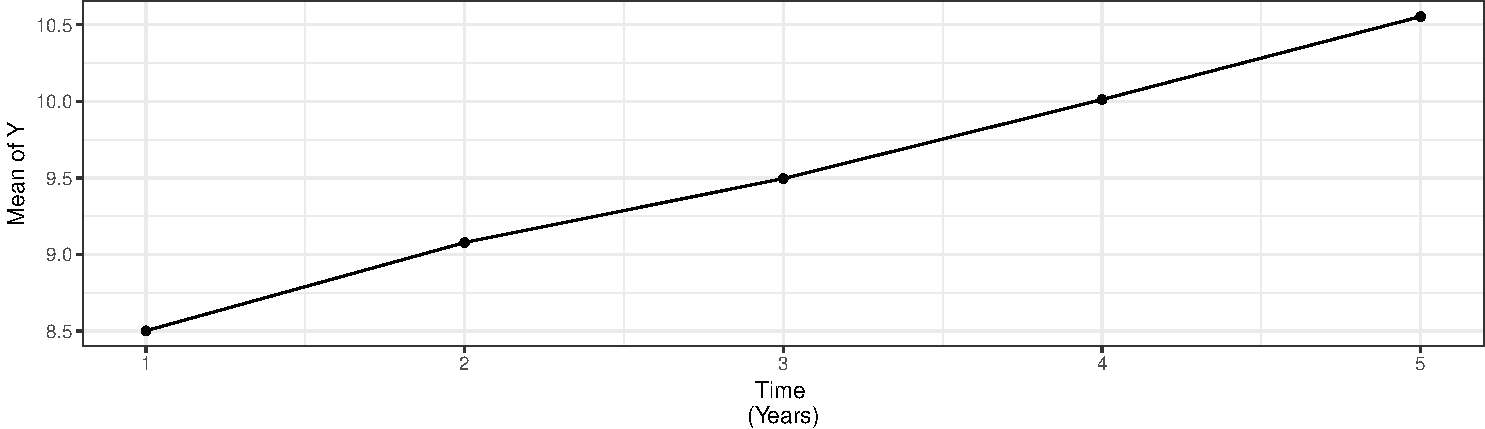
\includegraphics{r-tutorial_files/figure-beamer/unnamed-chunk-12-1.pdf}

\normalsize

\end{frame}

\begin{frame}[fragile]{Visualization in ggplot2 (cont.)}

We will now visualize the relationship between \(Y\) and \(X\), using it
as an opportunity to show off some of the customization available in
\texttt{ggplot2}:

\footnotesize

\begin{Shaded}
\begin{Highlighting}[]
\NormalTok{ggp_X <-}\StringTok{ }\KeywordTok{ggplot}\NormalTok{(}\KeywordTok{aes}\NormalTok{(}\DataTypeTok{x =} \NormalTok{X_quantile_bin, }\DataTypeTok{y =} \NormalTok{Y_mean), }\DataTypeTok{data =} \NormalTok{Y_X_stats) +}
\StringTok{  }\KeywordTok{geom_point}\NormalTok{(}\KeywordTok{aes}\NormalTok{(}\DataTypeTok{size =} \NormalTok{count), }\DataTypeTok{shape =} \DecValTok{1}\NormalTok{) +}\StringTok{ }\CommentTok{# circles that scale with count}
\StringTok{  }\KeywordTok{geom_line}\NormalTok{() +}\StringTok{ }\CommentTok{# this says to display a line}
\StringTok{  }\KeywordTok{geom_vline}\NormalTok{(}\DataTypeTok{xintercept =} \NormalTok{.}\DecValTok{5}\NormalTok{, }\DataTypeTok{linetype =} \StringTok{"dashed"}\NormalTok{) +}\StringTok{ }\CommentTok{# vertical line at median}
\StringTok{  }\KeywordTok{annotate}\NormalTok{(}\StringTok{"text"}\NormalTok{, }\DataTypeTok{x =} \NormalTok{.}\DecValTok{46}\NormalTok{, }\DataTypeTok{y =} \FloatTok{10.2}\NormalTok{, }\DataTypeTok{label =} \StringTok{"Median"}\NormalTok{) +}\StringTok{ }\CommentTok{# annotate median}
\StringTok{  }\KeywordTok{theme_bw}\NormalTok{() +}\StringTok{ }\CommentTok{# attractive black-and-white color scheme}
\StringTok{  }\KeywordTok{labs}\NormalTok{(}\DataTypeTok{size =} \StringTok{"Obs. Count"}\NormalTok{) +}\StringTok{ }\CommentTok{# set legend title}
\StringTok{  }\KeywordTok{ylab}\NormalTok{(}\KeywordTok{expression}\NormalTok{(Mean ~}\StringTok{ }\NormalTok{of ~}\StringTok{ }\NormalTok{Y[it])) +}\StringTok{ }\CommentTok{# math label}
\StringTok{  }\KeywordTok{xlab}\NormalTok{(}\KeywordTok{expression}\NormalTok{(Quantile ~}\StringTok{ }\NormalTok{Bin ~}\StringTok{ }\NormalTok{of ~}\StringTok{ }\NormalTok{X[it])) }\CommentTok{# math label}
\NormalTok{ggp_X }\CommentTok{# print figure}
\end{Highlighting}
\end{Shaded}

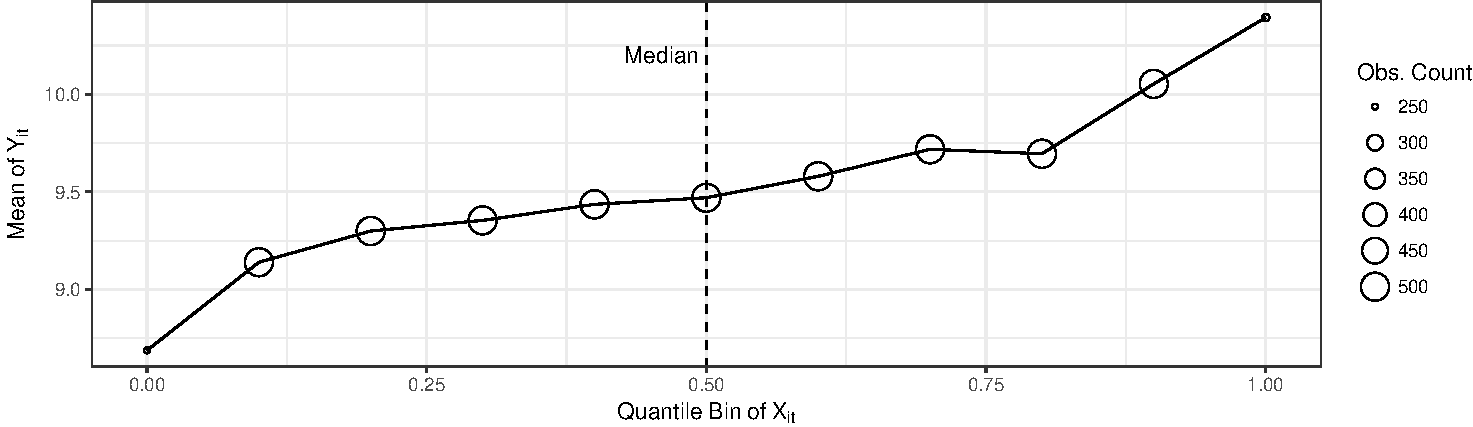
\includegraphics{r-tutorial_files/figure-beamer/unnamed-chunk-13-1.pdf}

\normalsize

\end{frame}

\begin{frame}[fragile]{Regression Analysis: OLS using lm}

Now suppose we wish to estimate \(\beta\), which is 1 in the simulation.
We will use \texttt{lm} (``linear model'') and R's regression formula
notation:

\footnotesize

\begin{Shaded}
\begin{Highlighting}[]
\NormalTok{OLS_formula_base <-}\StringTok{ }\KeywordTok{as.formula}\NormalTok{(}\StringTok{"Y ~ X"}\NormalTok{) }\CommentTok{# define the formula}
\NormalTok{OLS_result_base <-}\StringTok{ }\KeywordTok{lm}\NormalTok{(}\DataTypeTok{formula =} \NormalTok{OLS_formula_base, }\DataTypeTok{data =} \NormalTok{obsdata) }\CommentTok{# regression}
\NormalTok{OLS_coef_base <-}\StringTok{ }\KeywordTok{coef}\NormalTok{(}\KeywordTok{summary}\NormalTok{(OLS_result_base)) }\CommentTok{# extract results as matrix}
\NormalTok{OLS_coef_base }\CommentTok{# print results}
\end{Highlighting}
\end{Shaded}

\begin{verbatim}
##              Estimate Std. Error   t value     Pr(>|t|)
## (Intercept) 9.8629647 0.03010966 327.56815 0.000000e+00
## X           0.2314779 0.01417932  16.32503 2.078508e-58
\end{verbatim}

\normalsize

The coefficient on \(X\), 0.23, should have been 1, so OLS is
downward-biased. Now let's try controlling for a linear time trend:

\footnotesize

\begin{Shaded}
\begin{Highlighting}[]
\NormalTok{OLS_formula_time <-}\StringTok{ }\KeywordTok{as.formula}\NormalTok{(}\StringTok{"Y ~ X + time"}\NormalTok{) }\CommentTok{# define the formula}
\NormalTok{OLS_result_time <-}\StringTok{ }\KeywordTok{lm}\NormalTok{(}\DataTypeTok{formula =} \NormalTok{OLS_formula_time, }\DataTypeTok{data =} \NormalTok{obsdata) }\CommentTok{# regression}
\NormalTok{OLS_coef_time <-}\StringTok{ }\KeywordTok{coef}\NormalTok{(}\KeywordTok{summary}\NormalTok{(OLS_result_time)) }\CommentTok{# extract results as matrix}
\NormalTok{OLS_coef_time }\CommentTok{# print results}
\end{Highlighting}
\end{Shaded}

\begin{verbatim}
##              Estimate Std. Error   t value Pr(>|t|)
## (Intercept) 7.9839016 0.04012428 198.97930        0
## X           0.5558655 0.01235384  44.99534        0
## time        0.7826190 0.01359122  57.58269        0
\end{verbatim}

\normalsize

\end{frame}

\begin{frame}[fragile]{Regression Analysis: Fixed Effects using lm and
felm}

The coefficient estimate on \(X\) is downward-biased because \(X_{i,t}\)
is negatively correlated with the fixed effect \(\mu_i\). We can control
for the fixed effect in OLS by including a factor indicator for each id:

\footnotesize

\begin{Shaded}
\begin{Highlighting}[]
\NormalTok{OLS_formula_fe <-}\StringTok{ }\KeywordTok{as.formula}\NormalTok{(}\StringTok{"Y ~ X + time + as.factor(id)"}\NormalTok{) }\CommentTok{# define the formula}
\NormalTok{OLS_result_fe <-}\StringTok{ }\KeywordTok{lm}\NormalTok{(}\DataTypeTok{formula =} \NormalTok{OLS_formula_fe, }\DataTypeTok{data =} \NormalTok{obsdata) }\CommentTok{# regression}
\NormalTok{OLS_coef_fe <-}\StringTok{ }\KeywordTok{coef}\NormalTok{(}\KeywordTok{summary}\NormalTok{(OLS_result_fe)) }\CommentTok{# extract results as matrix}
\NormalTok{OLS_coef_fe[}\DecValTok{1}\NormalTok{:}\DecValTok{3}\NormalTok{, ] }\CommentTok{# too much output to show everything}
\end{Highlighting}
\end{Shaded}

\begin{verbatim}
##             Estimate Std. Error  t value     Pr(>|t|)
## (Intercept) 7.797695 0.43736076 17.82898 1.768675e-68
## X           1.038548 0.01535736 67.62544 0.000000e+00
## time        1.024771 0.01243031 82.44134 0.000000e+00
\end{verbatim}

\normalsize

This is the right answer! However, it requires a variable for each
individual, so it is infeasible for big data. Use \texttt{felm} from
\emph{lfe} for big data:

\footnotesize

\begin{Shaded}
\begin{Highlighting}[]
\KeywordTok{library}\NormalTok{(lfe)}
\NormalTok{felm_formula <-}\StringTok{ }\KeywordTok{as.formula}\NormalTok{(}\StringTok{"Y ~ X + time | id"}\NormalTok{) }\CommentTok{# define the formula}
\NormalTok{felm_result <-}\StringTok{ }\KeywordTok{felm}\NormalTok{(}\DataTypeTok{formula =} \NormalTok{felm_formula, }\DataTypeTok{data =} \NormalTok{obsdata) }\CommentTok{# regression}
\NormalTok{felm_result }\CommentTok{# use felm_result$STATS to see all the output}
\end{Highlighting}
\end{Shaded}

\begin{verbatim}
##     X  time 
## 1.039 1.025
\end{verbatim}

\normalsize

\end{frame}

\begin{frame}[fragile]{Importing and Exporting}

R has many available file formats for reading and writing data.

\begin{itemize}
\tightlist
\item
  In general, always try to use CSV. CSV files are lightweight and can
  be written and read by any other language (Stata, Python, Excel, etc).
\item
  In the rare event that you need to save a full list structure, use RDS
  files to save lists one at a time. These can only be openend by R.
\item
  Try to never use RData or save a workspace. This is prone to generate
  conflicts in your workspace since it can include any objects,
  including objects you did not mean to save or load.
\end{itemize}

Here is an example of writing and then reading the observed data as CSV:

\footnotesize

\begin{Shaded}
\begin{Highlighting}[]
\CommentTok{# Write to CSV. Always omit row names and replace missings with a space.}
\KeywordTok{write.csv}\NormalTok{(obsdata, }\DataTypeTok{file =} \StringTok{"observed_data.csv"}\NormalTok{, }\DataTypeTok{row.names =} \NormalTok{F, }\DataTypeTok{na =} \StringTok{" "}\NormalTok{)}
\CommentTok{# Read data from CSV and immediately set it as a data.table.}
\NormalTok{obsdata <-}\StringTok{ }\KeywordTok{setDT}\NormalTok{(}\KeywordTok{read.csv}\NormalTok{(}\DataTypeTok{file =} \StringTok{"observed_data.csv"}\NormalTok{))}
\end{Highlighting}
\end{Shaded}

\normalsize

Here is how to save a ggplot2 object as a PDF figure:

\footnotesize

\begin{Shaded}
\begin{Highlighting}[]
\KeywordTok{ggsave}\NormalTok{(ggp_time, }\DataTypeTok{file =} \StringTok{"ggplot_time.pdf"}\NormalTok{, }\DataTypeTok{height =} \DecValTok{5}\NormalTok{, }\DataTypeTok{width =} \DecValTok{8}\NormalTok{)}
\end{Highlighting}
\end{Shaded}

\normalsize

\end{frame}

\begin{frame}[fragile]{Quiz \#2: Data Analysis and Visualization}

Simulate data again from the model:

\[
Y_{i,t} = \alpha + \beta X_{i,t} + t\kappa  + \mu_i + \epsilon_{i,t}.
\]

Instead of being iid, let \(X_{i,t}\) also depends on
\(\epsilon_{i,t}\). Furthermore, draw an observed variable \(Z_{i,t}\)
which is independent of \(\epsilon_{i,t}\), and have \(X_{i,t}\) also
depend on \(Z_{i,t}\). The observed data is now
\((Y_{i,t},X_{i,t},Z_{i,t})\).

Demonstrate how to estimate \(\beta\) using the command \texttt{ivreg}
from package \emph{AER}, where we treat \(X_{i,t}\) as the endogenous
variable and \(Z_{i,t}\) as the instrumental variable.

Then, use felm to estimate the same instrumental variables regression
more efficiently. {[}Hint: In felm, the instrumental variables notation
looks like
\texttt{felm\_formula\ \textless{}-\ as.formula("Y\ \textasciitilde{}\ time\ \textbar{}\ id\ \textbar{}\ (X\ \textasciitilde{}\ Z)")}.{]}

Finally, export the matrix of regression coefficients, standard errors,
and p-values from ivreg and felm as CSV file. {[}Note that ivreg and
felm organize their results somewhat differently.{]}

\end{frame}

\section{III. Style and Structure
Rules}\label{iii.-style-and-structure-rules}

\begin{frame}{Overview}

The tidyverse coding style, which is derived from Google's R style
guide, is available here: \url{http://style.tidyverse.org/}. However, it
does not cover issues of scoping or when to check for errors, which are
key.

Note: The \emph{styler} package can re-write your code to satisfy the
style guide. It does things like automatically replace equals (a = 3)
with arrows (a \textless{}- 3), and replace single quotes (`hello') with
double quotes (``hello''). It has an RStudio plug-in for ease of use. I
highly recommend using styler, especially when you are new to R and
still learning its style. (All of my code here was edited by styler.)

On the next few slides, I will cover what I consider to be the 3 most
important rules of R style and organization:

\begin{enumerate}
\def\labelenumi{\arabic{enumi}.}
\tightlist
\item
  Use informative names;
\item
  Manually control function scoping; and,
\item
  Fill functions with manual error checks.
\end{enumerate}

\end{frame}

\begin{frame}[fragile]{Rule \#1: Use informative names}

Consider the function that calculates the rents collected by workers in
the Lamadon, Mogstad, and Setzler (2018) model using the wages and the
preference parameter \(\beta\). You could write this as:

\footnotesize

\begin{Shaded}
\begin{Highlighting}[]
\NormalTok{function1 <-}\StringTok{ }\NormalTok{function(x, y) \{}
  \KeywordTok{return}\NormalTok{(x /}\StringTok{ }\NormalTok{(}\DecValTok{1} \NormalTok{+}\StringTok{ }\NormalTok{y))}
\NormalTok{\}}
\end{Highlighting}
\end{Shaded}

\normalsize

It is difficult to see how this relates to the worker rents formula.
Try:

\footnotesize

\begin{Shaded}
\begin{Highlighting}[]
\NormalTok{compute_worker_rents <-}\StringTok{ }\NormalTok{function(sum_of_wages, beta_preference) \{}
  \KeywordTok{return}\NormalTok{(sum_of_wages /}\StringTok{ }\NormalTok{(}\DecValTok{1} \NormalTok{+}\StringTok{ }\NormalTok{beta_preference))}
\NormalTok{\}}
\end{Highlighting}
\end{Shaded}

\normalsize

Two other notes on names:

\begin{itemize}
\tightlist
\item
  Multiple words in a name should be separate by the underscore
  (worker\_rents) rather than the dot (worker.rents).
\item
  Do not re-use names. For example, ``c'' is used to make vectors, so
  don't call any of your variables c.
\end{itemize}

\end{frame}

\begin{frame}[fragile]{Rule \#2: Manually control function scoping}

When a function requires a variable that is not passed into the function
as an argument, it will search outside of the function into the next
highest scope. This can be very dangerous. Here is an example (courtesy
of Darren Wilkinson's blog):

\footnotesize

\begin{Shaded}
\begin{Highlighting}[]
\NormalTok{a <-}\StringTok{ }\DecValTok{1}
\NormalTok{f <-}\StringTok{ }\NormalTok{function(x) \{}
  \KeywordTok{return}\NormalTok{(a *}\StringTok{ }\NormalTok{x)}
\NormalTok{\}}
\NormalTok{g <-}\StringTok{ }\NormalTok{function(x) \{}
  \NormalTok{a <-}\StringTok{ }\DecValTok{2}
  \KeywordTok{return}\NormalTok{(}\KeywordTok{f}\NormalTok{(x))}
\NormalTok{\}}
\KeywordTok{g}\NormalTok{(}\DecValTok{3}\NormalTok{)}
\end{Highlighting}
\end{Shaded}

\begin{verbatim}
## [1] 3
\end{verbatim}

\normalsize

I wanted a=2 to be true when g(3) is evaluated on the last line, but
f(x) searched for a in the wrong scope and used a=1 instead.

\end{frame}

\begin{frame}[fragile]{Rule \#2: Manually control function scoping
(cont.)}

There are a number of ways to prevent the mistake on the previous slide,
but the simplest and most reliable way is to pass 100\% of objects used
by the function as function arguments:

\footnotesize

\begin{Shaded}
\begin{Highlighting}[]
\NormalTok{a <-}\StringTok{ }\DecValTok{1}
\NormalTok{f <-}\StringTok{ }\NormalTok{function(x, a) \{}
  \KeywordTok{return}\NormalTok{(a *}\StringTok{ }\NormalTok{x)}
\NormalTok{\}}
\NormalTok{g <-}\StringTok{ }\NormalTok{function(x) \{}
  \NormalTok{a <-}\StringTok{ }\DecValTok{2}
  \KeywordTok{return}\NormalTok{(}\KeywordTok{f}\NormalTok{(x, a))}
\NormalTok{\}}
\KeywordTok{g}\NormalTok{(}\DecValTok{3}\NormalTok{)}
\end{Highlighting}
\end{Shaded}

\begin{verbatim}
## [1] 6
\end{verbatim}

\normalsize
Now that f includes a as an argument, there is no problem. 100\% of
objects used in a function should be passed into it as arguments.

\end{frame}

\begin{frame}[fragile]{Rule \#3: Fill functions with manual error
checks}

Here, I will make two mistakes:

\footnotesize

\begin{Shaded}
\begin{Highlighting}[]
\NormalTok{f <-}\StringTok{ }\NormalTok{function(data, a) \{}
  \NormalTok{data[, var2 :}\ErrorTok{=}\StringTok{ }\NormalTok{a]}
  \KeywordTok{return}\NormalTok{(data)}
\NormalTok{\}}
\NormalTok{dd <-}\StringTok{ }\KeywordTok{data.table}\NormalTok{(}\DataTypeTok{var1 =} \KeywordTok{c}\NormalTok{(}\DecValTok{1}\NormalTok{, }\DecValTok{2}\NormalTok{))}
\KeywordTok{f}\NormalTok{(data, }\DataTypeTok{a =} \DecValTok{2}\NormalTok{) }\CommentTok{# I meant to write data=dd here!}
\end{Highlighting}
\end{Shaded}

\begin{verbatim}
## Error in `:=`(var2, a): Check that is.data.table(DT) == TRUE. Otherwise, := and `:=`(...) are defined for use in j, once only and in particular ways. See help(":=").
\end{verbatim}

\begin{Shaded}
\begin{Highlighting}[]
\KeywordTok{f}\NormalTok{(}\DataTypeTok{data =} \NormalTok{dd, }\DataTypeTok{a =} \KeywordTok{c}\NormalTok{(}\DecValTok{2}\NormalTok{, }\DecValTok{3}\NormalTok{, }\DecValTok{4}\NormalTok{)) }\CommentTok{# a has too many numbers here!}
\end{Highlighting}
\end{Shaded}

\begin{verbatim}
## Warning in `[.data.table`(data, , `:=`(var2, a)): Supplied 3 items to be
## assigned to 2 items of column 'var2' (1 unused)
\end{verbatim}

\normalsize

\begin{itemize}
\tightlist
\item
  Why doesn't the first error just say
  \texttt{"data\ does\ not\ exist"}? It turns out this is because
  \texttt{data} is a function in base R, so \texttt{data} actually
  already exists! (If I had known this, I would not have called the
  object \texttt{data}, per Rule \#1 above.)
\item
  Why does the second give a warning instead of an error? This is an
  example of R trying to help but causing a disaster!
\end{itemize}

\end{frame}

\begin{frame}[fragile]{Rule \#3: Fill functions with manual error checks
(cont.)}

\footnotesize

\begin{Shaded}
\begin{Highlighting}[]
\NormalTok{f <-}\StringTok{ }\NormalTok{function(data, a) \{}
  \NormalTok{if (!}\KeywordTok{is.data.table}\NormalTok{(data)) \{}
    \KeywordTok{stop}\NormalTok{(}\KeywordTok{sprintf}\NormalTok{(}\StringTok{"Input `data` must be data.table but is %s.}\CharTok{\textbackslash{}n}\StringTok{"}\NormalTok{, }\KeywordTok{class}\NormalTok{(data)))}
  \NormalTok{\}}
  \NormalTok{if (!}\KeywordTok{is.numeric}\NormalTok{(a)) \{}
    \KeywordTok{stop}\NormalTok{(}\KeywordTok{sprintf}\NormalTok{(}\StringTok{"Input `a` must be numeric but is %s.}\CharTok{\textbackslash{}n}\StringTok{"}\NormalTok{, }\KeywordTok{class}\NormalTok{(a)))}
  \NormalTok{\}}
  \NormalTok{if (!(}\KeywordTok{length}\NormalTok{(a) ==}\StringTok{ }\DecValTok{1} \NormalTok{|}\StringTok{ }\KeywordTok{length}\NormalTok{(a) ==}\StringTok{ }\KeywordTok{nrow}\NormalTok{(data))) \{}
    \KeywordTok{stop}\NormalTok{(}\KeywordTok{sprintf}\NormalTok{(}
      \StringTok{"Input `a` is of length %i }\CharTok{\textbackslash{}n}\StringTok{while input `data` is of length %i.}\CharTok{\textbackslash{}n}\StringTok{"}\NormalTok{,}
      \KeywordTok{length}\NormalTok{(a), }\KeywordTok{nrow}\NormalTok{(data)}
    \NormalTok{))}
  \NormalTok{\}}
  \NormalTok{data[, var2 :}\ErrorTok{=}\StringTok{ }\NormalTok{a]}
  \KeywordTok{return}\NormalTok{(data)}
\NormalTok{\}}
\NormalTok{dd <-}\StringTok{ }\KeywordTok{data.table}\NormalTok{(}\DataTypeTok{var1 =} \KeywordTok{c}\NormalTok{(}\DecValTok{1}\NormalTok{, }\DecValTok{2}\NormalTok{))}
\KeywordTok{f}\NormalTok{(data, }\DataTypeTok{a =} \DecValTok{2}\NormalTok{)}
\end{Highlighting}
\end{Shaded}

\begin{verbatim}
## Error in f(data, a = 2): Input `data` must be data.table but is function.
\end{verbatim}

\begin{Shaded}
\begin{Highlighting}[]
\KeywordTok{f}\NormalTok{(}\DataTypeTok{data =} \NormalTok{dd, }\DataTypeTok{a =} \KeywordTok{c}\NormalTok{(}\DecValTok{2}\NormalTok{, }\DecValTok{3}\NormalTok{, }\DecValTok{4}\NormalTok{))}
\end{Highlighting}
\end{Shaded}

\begin{verbatim}
## Error in f(data = dd, a = c(2, 3, 4)): Input `a` is of length 3 
## while input `data` is of length 2.
\end{verbatim}

\normalsize

\end{frame}

\begin{frame}[fragile]{Quiz \#3: Style and Structure}

Rewrite the codes you wrote for Quiz \#1 and \#2 to satisfy all of the
style and structure rules. {[}Hint: the \texttt{style\_active\_file()}
function from the \emph{styler} package can do a lot of the work.{]}

Save these as separate files so you can compare before/after.

Note that coming up with useful error checks is as much an art as a
science, as you need to anticipate possible mistakes you or another user
could make.

\end{frame}

\section{IV. Developing a Package (IN
PROGRESS)}\label{iv.-developing-a-package-in-progress}

\begin{frame}{Why Use Packages?}

\begin{itemize}
\item
  Objects are organized and updated to the latest version;
\item
  Objects are documented so you know what they do;
\item
  Clear separation of the tools (what you use) from the application
  (what you're analyzing with those tools);
\item
  Reproducibility since anyone can install/test the package;
\item
  Nice structure/methods for testing that the tools work.
\end{itemize}

\end{frame}

\begin{frame}{Creating a .RProject and Organizing Package Contents}

This is easy with RStudio.

\end{frame}

\begin{frame}{Writing Documentation}

Example of function with documentation:

Later, we will use the command roxygenize() from the package roxygen2 to
compile the documentation.

\end{frame}

\begin{frame}{Building, checking, compiling, and installing}

\end{frame}

\begin{frame}{Quiz on Package Development}

\end{frame}

\end{document}
